\subsection{Altérations, pertes et déplacements dans la tradition manuscrite}

Une œuvre copiée dans un manuscrit ou dans un livre imprimé peut subir des changements significatifs au fil du temps.

Durant sa copie ou son impression, des erreurs ou des corrections peuvent se glisser dans le texte ou les diagrammes.

Les éléments iconographiques peuvent aussi avoir des changements dans leur style, leur contenu et la propreté de réalisation, ce qui peut rendre l'identification difficile même pour un spécialiste. 

En ce qui concerne l'organisation du manuscrit ou du livre imprimé, les feuillets et les cahiers sont parfois changés de place, voire perdu. Cela complique la comparaison car l'ordre des images est se retrouve aussi perturbé. 

Il arrive également que les images soient retouchées ou ajoutée ultérieurement par une autre main que celui du copiste originel. Cette action doit être prise en compte car elle est intéressante pour la transmission d'un savoir au fil des temps. Cependant, elle peut aussi porter à confusion si nous n'arrivons pas à détecter qu'elle ait été ajouté bien plus tard.

Le problème le plus grave que nous pouvons rencontrer est la dégradation de l'ouvrage dans le temps. Saito évoque dans son article sur l'évolution des éditions d'Euclide au fil du temps qu'un manuscrit qu'il désigne sous le nom de \og manuscrit F \fg seraient l'une des meilleures lectures d'une partie de l'œuvre mais malheureusement elle est très endommagée ce qui complique sa lecture. CITER SAITO Dans le cas des diagrammes, il n'est pas rare que les encres se détériorent et deviennent difficile à comprendre. La dégradation du support rend la lecture compliquée et peut impacter son utilisation dans une étude philologique.

La pire situation qu'il puisse arriver à un ouvrage est évidemment sa perte qui rend son exploitation impossible.



\subsection{Les différentes conventions de représentation d'un diagramme}

Le travail de l'historien des sciences peut s'avérer compliqué lorsqu'un concept ou une démonstration est représentée de manière différente. En effet, les conventions et les choix graphiques diffèrent en fonction de l'époque, de l'endroit et du sujet d'étude comme c'est le cas avec les diagrammes.

Michela Malpangotto étudie ce phénomène en s'appuyant sur l'exemple de l'œuvre de Théodose les \textit{Sphériques} écrite au Ier siècle avant notre ère. Il s'agit d'un texte fondamental dans l'étude de la géométrie sphérique qui est structuré en 59 propositions et divisé en trois livres. Il fait partie de ce que l'on nomme la \og Petite astronomie \fg, un recueil d'ouvrages compilés par les Grecs afin de faciliter la compréhension de l'\textit{Almageste} de Ptolémée. Il a été étudié et transmis pendant près de dix siècles. La géométrie sphérique est définie de la manière suivante : \og La géométrie sphérique étudie la sphère comme un objet solide mais surtout comme contexte spatial des éléments qui interagissent sur elle dans un agencement tridimensionnel complexe. \fg Il est alors nécessaire de mettre au même niveau, le plan du diagramme et l'agencement spatial des objets autour de la sphère. Cette dernière est un objet solide mais elle est surtout un contexte spatial pour des arcs, des segments de droites et des cercles qui y sont déterminés par l'intersection de différents plans inclinés dans l'agencement spatial tridimensionnel. Cependant, le concept de sphère n'est pas représenté de la même manière chez tous les auteurs. 

Dans la version grecque originale, illustré ici par le manuscrit Vat. Gr. 204, les deux parties de l'œuvre sont séparées par le choix de l'iconographie des diagrammes. Dans la première partie, nous retrouvons des diagrammes dans lesquelles la sphère n'est pas représentée. Il y a seulement des cercles produits par l'intersection du plan incliné de différentes façons qui sont représentés de manière juxtaposés dans le plan du diagrammes. Les arcs ainsi que les segments linaires sont aplatis et les objets placés de l'autre côté de la sphères sont retournés dans le plan de la figure. La conséquence majeure de ce mode de représentation est la dépendance des diagrammes vis-à-vis du texte. Il est nécessaire de lire les explications pour comprendre le diagramme. Dans la seconde partie de l'œuvre, les diagrammes sont construits en utilisant la perspective. Nous pouvons donc observer les éléments géométriques interagir entre eux à l'intérieur de cette dernière.  

En Italie, Platon de Tivoli a réalisé trois éditions de cette œuvre au XVIe siècle en s'appuyant sur une version arabo-latine médiévale. Il choisit de représenter les diagrammes de manière schématique et plane comme dans la première partie de la version grecque originale de l'œuvre. 

L'édition de Francesco Maurolico marque un tournant dans la transmission des \textit{Sphériques}. En effet, ce dernier fait le choix de travailler sur la surface de la sphère qui, mise en avant, devient le contexte réel dans lequel les éléments géométriques interagissent. Christophe Clavius, un mathématicien allemand adopte cette iconographie dans son édition de 1586 qui sert de base à la tradition moderne des \textit{Sphériques}\footcite{malpangottoGraphicalChoicesGeometrical2010}. 

\begin{figure}[h]
	\centering
	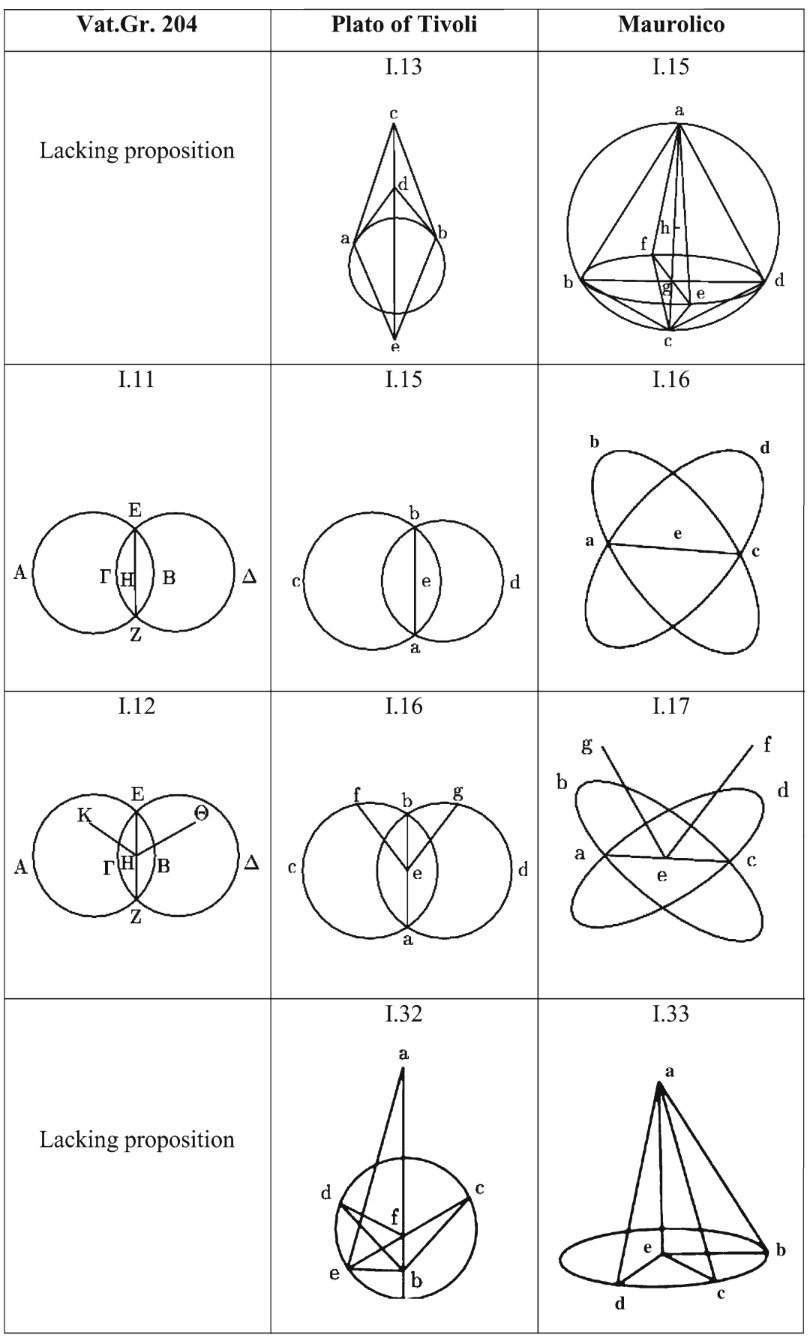
\includegraphics[width=0.9\linewidth]{images/conventions_diagrammes.png}
	\caption{Différentes conventions de représentation de diagrammes évoquées par Michela Malpangotto\footcite{malpangottoGraphicalChoicesGeometrical2010}}
	\label{fig:conventions}
\end{figure}


L'étude de Michela Malpangotto nous montre l'existence de nombreuses conventions graphiques de diagrammes pouvant être très différentes en fonction des éditeurs et des époques. Lorsque nous tentons de retracer la diffusion d'une œuvre à partir de ces diagrammes, il est important de prendre en compte ce paramètre. Néanmoins, ces différentes manières de représenter les diagrammes sont aussi en elles-mêmes les témoins de l'évolution d'un concept et donc par extension des connaissances scientifiques.

\subsection{La modification des diagrammes dans les éditions modernes des sources scientifiques}

Les modifications que s'autorisent de faire les philologues et éditeurs contemporains peuvent rendre la comparaison avec les sources anciennes compliquée. Dans un article, Saito étudie les éditions modernes des diagrammes astronomiques des Elements d'Euclide. Il expose la problématique suivante : les diagrammes que nous voyons dans les éditions imprimées à partir du XIXe siècle sont très différents de ceux présents dans les manuscrits médiévaux. Pourtant ces derniers sont les meilleures versions, voire les seules témoins des œuvres antique mathématiques en absence de manuscrit datant de cette époque. La version qui sert de base à beaucoup d'éditions contemporaines (A VERIFIER) est celle d'Heiberg datant de 1883-1888. Cependant, ce dernier s'est contenté de copier les diagrammes d'Auguste simplifiés dans un but pédagogique datant des années 1820. Se pose alors la question des conventions d'édition. Deux points de vue s'opposent alors. Nous avons d'abord celui de la maison d'édition Les Belles Lettres décrit dans leur \textit{Règles et recommandations pour les éditions critiques} qui explique qu'il est nécessaire de reproduire les diagrammes aussi précisément que possible sans essayer de les corriger ou modifier. Michael Hunter, lui, défend plutôt l'idée selon laquelle il est acceptable que des diagrammes soient redessinés pour que l'intention originelle de l'auteur soit transmise au lecteur. JARDINE

Lorsque nous nous penchons sur une édition moderne d'un texte scientifique il faut alors prendre en compte les modifications possibles des diagrammes par rapport aux œuvres originales. Il s'agit d'une bonne raison pour repenser sa manière de réaliser des éditions critiques en tentant d'être le plus proche possible de l'œuvre originale. Pour éviter de se tourner directement vers des versions de l'œuvre déjà éditées, il serait préférable de revenir aux sources médiévales et modernes en utilisant de nouveaux outils numériques pour faciliter l'exploration et l'analyse de centaines de témoins disponibles en ligne avec une dimension collaborative du travail. A REFORMULER